\chapter{Проектиране на система за езиково обучение}
\section{Преглед на системата}
\subsection{Функционалност}
Всяка система за езиково обучение трябва да предлага минимум речников
модул, различни изпитни модули и модули за упражнение и затвърждаване
на знания. Изпитните модули, обикновено, биват
изградени върху думите налични в речниковата база на приложението и
допълнителна метаинформация за тях. 

В Spellbook речниковата база и метаинформацията, асоциирана с нея, се
съхраняват във вградена релационна база данни(H2). Това е голям
напредък от стандартното решение, езиковата база да се съхранява в
текстови файлове или в специално организирани двоични файлове по
няколко причини:
\begin{itemize}
  \item Имаме възможност за изключително ефективно търсене в базата -
    елиминира се нуждата от последователно обхождане на записи във файл
  \item Имаме възможост да моделираме данните в речниковата база, по
    начин, който отразява отношенията между тях(например един речник е
    изграден от думи и техните преводи на даден език или казано
    накратко - речникови записи)
  \item Имаме възможност лесно да манипулираме голям обем от данни
    едновременно
  \item Имаме възможност да използваме обектно-релационнен
    преобразувател като Hibernate, който да установи връзка между
    обектите в нашето приложение и данните в таблиците на базата данни.
\end{itemize}

Речниковият модул предоставя възможност за търсене на дефинициите на
думи в него. Търсенето може да е точно или приблизително, ако не бъде
открито точно съвпадение. Освен това речниковият модул е наясно с
връзките между наличните речници в речниковата база данни и поддържа
автоматично преключване между езиците в един
двупосочен(комплементарен) речник. За удобство на потребителите
речниковия модул трябва да поддържа интеграция с клипборда на
операционната система и история на търсените досега думи.

Стандартни изпитни модули в една система са превод на думи от един
език на друг и преговор на нови думи. Диктовките са сериозна част от
езиковата подготовка също. Модул за проверка на правописа обикновено служи
за тяхната проверка - ученикът просто копира текста, който той е
написал и моментално вижда броя на допуснатите от него грешки, както и
верните думи. В един по-комплексен сценарий, посредством интеграция със
сканиращо устройство и програма за разпознаване на текст може
ръкописни диктовки да бъдат дигитализирани от учениците и
преподавателите и проверени автоматично от системата. 

Научно доказано, е че човек(особено децата) усвояват материала, когато
той е поднесен забавно. Затова е от голямо значение някои от модулите
на системата да са организирани във вид на образователни игри.

Системата трябва да е изключително лесна за инсталиране и да не
изисква никаква начална конфигурация от своите
потребители. Настройките, зададени по подразбиране трябва да отговарят
на нуждите на голямата част от потребителите. В същото време системата
трябва да предлага високо ниво на гъвкавост - всички нейни по-ключови
аспекти трябва да се конфигурируеми. 

Системата трябва да е лесна за разширяване - добавянето на нови езици
в нея трябва да става по максимално прост начин. Освен това системата
трябва да дава възможност на потребителите си да я обогатят като
коригират грешки в речниковия фонд, разширяват речниковия фонд и
докладват грешки в системата и предложения за подобрения и нови
изпитни модули.

В ерата на Интернет и уеб базираните приложения е важно една такава
система да предлага както десктоп вариант, така и уеб вариант, за да
удовлетворява нуждите и предпочитанията на възможно най-голям брой
потребители. Двете приложения трябва да са тясно свързани и да работят
заедно за максимизиране на потенциала и възможностите им. 
\subsection{Езикова база данни}
Езиковата база данни е в основата на всички модули на системата. От
ключово значение е да бъде избран максимално добър формат за
съхранението на данните, който да гарантира бърз достъп до тях и
възможност за лесно разширяване на базата. 

Вградените релационните системи за управление на бази данни са
идеалното решение за такива ситуации. Те предлагат висока
производителност, малко потребеление на памет и голяма
гъвкавост. 

Езиковата база данни се състои от речников фонд и метаинформация за
думите(например честотата на срещането им в езика, правила за
образуване на множествено число) и езика(азбука, граматически
правила).

Подходящата метаинформация може да бъде използвана от различни модули
- например честотата на думите е един език може да бъде използвана от
изпитен модул за да разделя думите по трудност(по-рядко срещаните думи
се считат за по-трудни), а модула за проверка на правописа би
използвал честотата за генериране на списък с най-вероятните думи,
вместо сбърканата от вас.
\subsection{Комуникация с потребителите}
Потребителят винаги е прав и винаги знае от какво се нуждае системата,
тъй като реално той е този, който я използва. Разработчиците винаги
трябва да поддържат добро ниво на комуникация със своите потребители и
да се вслушват в техните критики и предложения. 

Системата представена в тази дипломна работа разполага с уеб сайт, на
който потребителите могат да маркират открити грешки и да споделят
предложения. Освен това системата разполага и с дискусионен списък,
където се обсъждат новите възможности на системата, цикъла на
разработка и други интересни неща от "`кухнята"' и. 

Интересни възможности са също така функционалност за автоматично
докладване на грешки, известяване за нови версии и т.н.
\subsection{Разпространение}
Всеки софтуерен продукт трябва евентуално да стигне до своите
потребители. Начините, по които това може да стане са разнообразни -
официалния сайт на проекта, алтернативни ftp и http сървъри, торент
тракери и т.н. 

Важно е да се обръща внимание на спецификата на операционната система
на потребителите, за да бъде инсталирането на софтуера максимално
удобно и интуитивно за тях. Въпреки, че софтуера написан на Java е
платформено независимим не трябва да забравяме някои неща:
\begin{itemize}
  \item За Windows потребителите е желателно да бъде предоставен
  инсталатор
  \item За потребителите на различните GNU/Linux дистрибуции е добре
    да бъдат предоставени специфичните пакети - например RPM за Red
    Hat базирани дистрибуции, deb за Debian базирани дистрибуции и
    т.н.
  \item За потребителите на OSX също трябва да бъде предоставена
    специална версия, лесна за инсталиране там
  \item За всички останали потребилите трябва да се предостави
    платформено архив, лесен за използване независимо от операционната система 
\end{itemize}
\section{Преглед на платформата и езика Java}
\subsection{Java като платформа за програмиране}
Първото издание на Java през 1996 г., генерира невероятна
възбуда, не само в компютърната преса, но в масовите медии като "`Ню
Йорк Таймс"', "`Вашингтон пост"', както и "`Седмица бизнес"'. Java има
честта да бъде  първият и единствен език за програмиране, на когото е
отделена десет минутна история по Националното обществено радио на САЩ. Сто
милиона щатски долара фонд за рисков капитал е създаден единствено за
продукти, произведени с използването на специфичен компютърен език.

Java безспорно е един добър език за програмиране, но неговата истинска
сила идва от Java платформата, която го заобикаля. Java никога не е
бил само език за програмиране. Има купища езици за програмиране, но
много малко от тях правят такова впечатление. Java е цяла платформа с
огромна библиотека, съдържаща много преизползваем код, с
инфраструктура за изпълнение, която предоставя сигурност, преносимост
между различните операционни системи и автоматично събиране на
боклука.

Програмистите желаят език с приятен и интуитивен синтаксис и
разбираема семантика. Java отговаря на това описание, но на него
отговарят още една дузина програмни езици. Някои от тях предлагат и
портативност и автоматично събиране на боклука, но нямат кой знае
каква стандартна библиотека и ви карат да правите много неща отначало
сами. Java ви предлага всичко - добър език, невероятна платформа за
изпълнение и огромна библиотека. Комбинацията от тези характеристики
прави Java неустоим избор за много програмисти по света и бе голям
фактор за избора на Java за реализацията на тази дипломна работа. 
\subsection{Ключови характеристики на Java}
Авторите на Java изтъкват 11 ключови характеристики на езика. В
следващите няколко реда съм изложил техните думи и кратък коментар:
\begin{itemize}
\item \textbf{Прост}
 
  \emph{Искахме да изградим система, която да може да бъде програмирана
    лесно без много допълнително обучение и която използва настоящите
    утвърдени практики. Въпреки, че С++ не отговаря на тази критерии,
    ние базирахме Java на него, доколкото бе възможно, за да направим
    системата по-лесна за разбиране. Java пропуска повечето рядко
    използвани, криво разбрани и объркващи възможности на C++, които
    смятаме, че носят повече проблеми, отколкото дивиденти.}

  Синтаксисът на Java наистина е изчистена версия на синтаксисът на
  C++. Няма нужда от заглавни файлове, указателна аритметика(или дори
  указателен синтаксис), структури, обединения, презареждане на
  оператори, виртуални базови класове и т.н. Дизайнерите на Java,
  обаче, не са се опитали да оправят всички проблемни неща в С++ -
  синтаксисът на твърдението switch например остава непроменен. Всеки,
  който владее С++ няма да има особени проблеми в прехода към Java.
  
  Аз самият направих преход именно от C++ към Java преди години и дори
  след толкова време не спирам да се впечатлявам от огромните
  предимства на Java спрямо C++ при наличието на толкова сходен
  синтаксис. Това за пореден път показва, че инфраструктурата зад един
  език е по-важна от самия език.
\item \textbf{Обектно ориентиран}

    \emph{Казано просто, обектно-ориентираният дизайн е техника за
    програмиране, при която фокусът е върху данните(обектите) и върху
    интерфейсите към тези обекти. Ако направим аналогия с
    дърводелството - един "`обектно-ориентиран"' дърводелец ще го е
    грижа повече за стола, който прави, като иструментите, с които
    работи са вторични. Един "`не-обектно-ориентиран"' дърводелец би
    мислил главно за инструментите си. Обектно-ориентираните пособия
    на Java са по същество същите като в С++.}

  Обектно ориентираното програмиране е доказало своите качества през
  последните 30 години и е почти немислимо модерен програмен език да не
  го използва(изключение, разбира се, са модерните функционални езици
  за програмиране). Наистина обектно-ориентираните характеристики на
  Java са сравними с тези на С++. Единствената по-голяма разлика, е че
  в Java множественото наследяване е заменено с по-простата концепция
  на интерфейси. Друга разлика е метаклас модела на Java.
  \item \textbf{Мрежов}

    \emph{Java има богата библиотека от процедури за работа с TCP/IP
    протоколи като HTTP и FTP. Java приложенията могат да отварят и
    достъпват обекти през Мрежата чрез URL със същата лекота, с която
    достъпват локалната файлова система.}

    Мрежовите възможности на Java са наистина големи и лесни за
    употреба. Всеки, който се е опитал да програмира за Интернет с някой
    друг език ще признае колко лесни са в Java сложни задачи, като
    отваряне на сокет връзка. Отдалеченото изпълняване на методи пък
    позволява комуникация между разпределени обекти.

  \item \textbf{Надежден}

    \emph{Java е предназначен за създаване на програми, които трябва да
    бъдат надеждни по различни параграфи. Java отдава голямо значение
    на ранното проверяване за потенциални проблеми, по-късното
    динамично(по време на изпълнение) проверяване и елеминирането на
    ситуации, които предразполагат към грешки. Най-голямата разлика
    между Java и C/C++ е, че Java има указателен модел, който
    елиминира възможността за презаписване на памет и повреждане на
    данни.}

  Тоза характеристика определено е много полезна. Java компилатора
  засича много проблеми, които в други езици биха се появили само по
  време на изпълнение на програмата. Колкото до втората точка от
  цитата - всеки, прекарал часове преследвайки проблем с паметта
  причинен от указател, ще е много щастлив в Java, поради
  невъзможността за възникване на подобни ситуации. 

  Интересен факт, е че указателният модел(а и концепцията за събиране
  на боклука) на Java съществува в Lisp още от далечната 1956
  година. Един от авторите на Java Гай Стийл(който същевременно е и
  един от създателите на Common Lisp) казва, че с Java авторите му са
  приближили C++ програмистите до средата на пътя към Lisp.

\item \textbf{Сигурен} 

  \emph{Java е предназначен за използване в мрежови/разпределени среди. В
  тази връзка, голямо внимание бе обърнато на сигурността. Java
  позволява създаването на системи без вируси, които е трудно да бъдат
  повлияни от недоброжелатели.}

От самото начало, Java е създадена да направи някои видове атаки
невъзможни. Сред тях са:

\begin{itemize}
\item Преливане на стека на изпълнение
\item Повреждане на паметта извън собственото адресно пространство
\item Четене и запис на файлове без необходитемите права
\end{itemize} 

В последствия в Java биват добавени още възможности в областта на
сигурността - например в Java 1.1 е добавена концепцията за цифрово
подписани класове, която дава сигурност кой точно е автора на даден клас.

  \item \textbf{Архитектурно неутрален}
    \emph{Компилаторът генерира архитектурно-неутрален обектен файлов
    формат. Компилираният код е изпълним на много процесори, при
    наличието на Java среда за изпълнение. Java компилатора постига
    това посредством генерирането на байткод инструкции, които нямат
    нищо общо с конкретната компютърна архитектура. Те са проектирани
    да бъдат лесни за интерпретиране и лесни за превеждане в машинен
    код по време на самото изпълнение.}

    Това определено не е нова идея - преди повече от 30 години Никлас
    Вирт използва този подход, когато създава оригиналната
    имплементация на Паскал. 

    Разбира се, интепретирането на байткод е по-бавно от изпълнението
    на машинни инструкции. За щастие, виртуалните машини имат
    способността да превеждат най-често използваните инструкции в
    машинен код, процес известен като "`компилация точно
    навреме"'(just in time). Тази стратегия се оказва толкова
    ефективна, че дори платформата .NET на Microsoft я
    използва. Използването на виртуална машина дава и други
    предимства. То повишава нивото на сигурност, тъй като виртуалната
    машина може да проверява поведението на последователност от
    инструкции. Някои програми дори произвеждат байткод динамично,
    разширявайки по този начин възможностите на работеща в момента
    програма.

  \item \textbf{Портативен}

    \emph{За разлика от C и С++, няма "`зависими от имплементацията"' аспекти на
      спецификацията. Размерите на примитивните типове данни са
      специфицирани, като и поведението на аритметиката с тях.}

    В Java int(целочислен примитивен тип) винаги е 32 битово цяло
    число. В C/C++ int може да означава 16 битово цяло число, 32
    битово цяло число, или друг размер, който е бил предпочетен от
    доставчика на компилатора. Единствената рестрикция, е че типа int
    трябва да има поне толкова байтове, колкото short int и, че не може
    да има повече байтове от long int. Наличието на фиксиран размер за
    числените типове елиминира огромни главоболия при пренасянето на
    едно приложение от една платформа на друга. Двоичните данни се
    съхраняват и пренасят във фиксиран формат, елиминирайки проблеми с
    подреждането на байтовете. Низовете се съхраняват в стандартен
    Unicode формат.

    \emph{Библиотеките, които са част от системата определят портативните
    интерфейси. Например имаме абстрактен клас Window и имплементации за
    него за UNIX, Windows и Macintosh.}

    Всеки, който го е опитвал, знае че са необходими усилия с героични
    пропорции да се напише програма, която изглежда добре на Windows,
    Macintosh и десет разновидности на UNIX. Java 1.0 направи това
    героично усилие, като достави набор от инструменти, който поддържаше
    елементи на потребителския интерфейс общи за няколко платформи. За
    съжаление, резултатът беше библиотека, която с много работа донасяше
    резултати, които бяха едва приемливи на различните системи. Но това
    беше някакво начало - има много приложения, за които преносимостта е
    по-ценна от добре изглеждащия потребителски интерфейс и тези
    приложения имаха полза дори от ранните версии на Java. В момента
    библиотеката за графични потребителски интерфейси е изцяло нова,
    написана отначало и вече не разчита на компонентите на
    системата-домакин. Резултата е много по-еднороден и много
    по-атрактивен от това, което ни предлагаха ранните версии на Java. 

  \item \textbf{Интепретиран}

    \emph{Java интерпретаторът може да изпълнява Java байткод директно на всяка
    една машина, за която същестува версия на интерпретатора. Тъй като
    свързването е по-инкрементален и лек процес, цялостният цикъл на
    разработка може да бъде по-бърз.}

    Инкременталното сврързване има предимства, но неговите предимства за
    процеса на разработка определено са по-скромни, отколкото твърдят
    авторите на Java. Ранните версии на Java инструментите за разработка
    бяха действително доста бавни. Днес, обаче, байткода се транслира в
    машинен код от JIT компилатор.
  \item \textbf{Високопроизводителен}

    \emph{Въпреки, че производителността на интерпретирания байткод е
    обикновено повече от адекватна, има ситуации, в които е необходима
    по-висока производителност. Байткод може да бъде транслиран в
    машинен код за сътвения процесор, върху който работи приложението,
    по време на изпълнение.}

    В ранните години на Java много потребители възразяваха с
    твърдението, че производителността е "`повече от
    адекватна"'. Днес, обаче, повечето JIT компилатори са толкова
    добри, че могат да се съзтезават успешно с традиционните
    компилатори и в някои ситуации, дори да предоставят по-голяма
    производителност, тъй като разполатат с повече
    информация. Например JIT компилатор може да следи кои сегменти от
    кода се изпълняват най-често и да ги оптимизира
    допълнително. По-комплексен пример е елиминирането на извиквания
    на методи(процес известен като вграждане). JIT компилатора знае
    кои класове са заредени. Той може да използва вграждане, когато
    базирано на заредените в момента класове определен метод не е
    презаписан и може да махне оптимизацията по-късно, ако това е необходимо.  

  \item \textbf{Многонишков}

       \emph{Предимствата на многонишковите програми са по-добра
       производителност и време за реакция.}

       Хората, писали многонишков код в други езици, вероятно ще
       останат приятно изненадани от това колко лесно става това в
       Java. Нишките в Java позволяват да се разгърне цялата мощ на
       многопроцесорна система, ако това се поддържа от операционната
       система. Негатив е, че нишковите имплементации на различните
       операционни системи се различават много и Java не се стреми да
       бъде платформено независима в тази насока. Само кода за
       извикване на многонишкови функции е един и също между
       различните платформи; Java делегира имплементацията на нишките
       на операционната система или на нишкова библиотека. Все пак
       леснотата, с която се работи с много нишки в Java, е една от
       ключовите му черти и една от основните причини да е
       предпочитана платформа за разработка на сървърни приложения.


  \item \textbf{Динамичен}

    \emph{В много отношения Java е по-динамичен език от С и С++. Той е
    проектиран да се адаптира към развиващи се среди. Библиотеките
    могат да добавят спокойно методи и полета без никакви ефекти върху
    техните клиенти. В Java намирането на информация за тип по време
    на изпълнението е просто.}

    Това е важна характеристика в случаите, когато код трябва да бъде
    добавен към работеща програма. Такъв пример е код, който се тегли
    от интернет и работи в браузър. В Java 1.0 намирането на типова
    информация по време на изпълнение определено не беше лесна
    задача. Текущите версии на Java, обаче, дават на програмистите
    достъп до структурата и поведението на обектите. Това е много
    полезно за приложения, които трябва да анализират обекти по време
    на изпълнение - дизайнери на графични интерфейси, дебъгери,
    включваеми компоненти и обектни бази данни.

\end{itemize}
\section{Преглед на Swing}
\subsection{Обзор}
Библиотеката Swing предоставя богат асортимент от компоненти за
изграждане на графични потребителски интерфейси и за добавяне на
интерактивност в Java приложения. Swing включва всички компоненти,
които бихте очаквали да откриете в една съвременна библиотека:
таблици, списъци, дървета, бутони и етикети.

Swing, обаче, далеч не е обикновена компонентна библиотека. Той
притежава отлична поддръжка на отмяна на действия и конфигурируем
текстов пакет, интернационализация и достъпност за хора с
увреждания. За да се възползва максимално от многоплатформените
възможности на Java, Swing поддържа много външни видове, както и
възможността да създадете ваш такъв, ако съществуващите не ви допадат.
Възможността за създаване на собствени външни видове е допълнително
улеснена от наличнието на Synth - външен вид специално създаден да
бъде персонализиран. Swing включва и поддръжка за drag and drop,
обработка на съобщения, специално изрисуване и управление на
прозорците.

Swing е част от Java Foundation Classes(JFC). JFC включва и други
възможности важни за едно графично приложение, като
способността да се добавят богата графична функционалност и да се
създаде програма, която работи на различни езици и приема вход от
различни входящи устройства.
\subsection{Възможности}
В следващите редове са изложени някои от основните възможности на
Swing и JFC.

\begin{itemize}
  \item \textbf{Swing графични компоненти}

    Библиотеката Swing включва в себе си богат набор от компоненти: от
    базови компоненти като бутони и полета за отметка, до комплексни
    компоненти като таблици и текст. Дори привидно прости компоненти
    като текстови полета, предлагат сериозни възможности, като
    форматиране на текста или поведение като поле за въвеждане на
    парола. Има файлови браузъри и диалози, които биха задоволили
    повечето нужди, в останалите случаи - възможни са промени. Ако
    никой от съществуващите компоненти не задоволява напълно нуждите ви
    лесно може да създадете свой.
  \item \textbf{Java 2D API}

    За да се подобри външния вид на едно приложение могат да бъдат
    добавени графики и анимации към потребителския интерфейс. Това
    става посредством Java 2D API. Тъй като Swing е изграден върху
    двуизмерния пакет, е тривиално да се използва двуизмерна графика в
    него. Добавянето на изображения, сенки, композитни графики и
    т.н. е лесно в Java 2D.
  \item \textbf{Включаеми външни видове(Pluggable Look and Feel)}
    
    Всяка програма, която използва Swing компоненти има възможността
    да избере външен вид. JFC, разработен от Sun и Apple включва външен
    вид, който наподобява ествествения такъв на платформата. Пакетът
    Synth позволява да създадете свой собствен външен вид. Външният
    вид GTK+ е отличен избор за приложения, които работят на GNU/Linux
    с GNOME.

    Една програма може да избере външния вид на платформата върху,
    която работи или някой Java външните видове(Metal, Nimbus) и без
    прекомпилиране програмата просто ще работи. Вие може спокойно да
    игнорирате този проблем и да оставите мениджъра на потребителския
    интерфейс да го разреши.
  \item \textbf{Трансфер на данни}
    
    Трансфер на данни посредством изрязване(cut), копиране(copy) и
    вмъкване(paste), както и влачене и пускане(drag and drop) е
    ключова възможност за почти всяко приложение. Поддръжката за
    трансфер на данни е вградена в Swing и работи между компонентите в
    едно приложение, между различни Java приложения и между Java и
    native(приложения, които директно използват системните библиотеки
    на операционната система)  приложения.
  \item \textbf{Интернационализация}

    Тази възможност позволява на разработчиците да изграждат
    приложения, които да комуникират с потребителите по целия свят на
    техните езици и съгласно техните културни конвенции. Могат да
    бъдат създадени приложения, които приемат като вход хиляди
    различни символи, като Японски, Китайски, Корейски.

    Мениджърите на разположението(layout manager) на Swing правят
    лесно създаването на определена ориентация изисквана от
    потребителския интерфейс. Например интерфейсът ще се появява от
    дясно на ляво, когато се използва локал, където текста се чете от
    дясно на ляво. Тази поддръжка е автоматична - трябва да напишете
    кода на интерфейса само веднъж и после той ще работи от дясно на
    ляво и от ляво на дясно, както и ще преоразмерява компонентите,
    които се променят, когато локализирате текст.
  \item \textbf{Достъпност}

    Инвалидите използват специални помощни софтуерни технологии, които
    посредничат между тях и приложението, което използват. Такъв
    софтуер се нуждае от много информация за работещото приложение, за
    да може да го представи в алтернативна форма. API на Java за
    достъпност реализира тези помощни технологии и им предоставя
    информацията, от която се нуждаят, както и възможността
    програматично да манипулират елементите, които изграждат графичния
    потребителски интерфейс.
  \item \textbf{Отмяна на действия}

    Частта от Swing посветена на "`отмяна"' позволява на програмистите
    да реализират действията "`отмени"'(undo) и "`направи
    отново"'(redo). Поддръжката за отмяна е вградена в текстовия компонент
    на Swing. За другите компоненти Swing поддържа неограничен брой
    действия, които могат да бъдат отменени и извършени отново.
  \item \textbf{Ръвкави схеми на експлоатация}

    Ако искате вашата програма да работи в уеб браузър може да я
    направите на аплет и да я изпълните чрез Java разширение, което
    поддържа разнообразни браузъри като Internet Explorer, Firefox,
    Safari, Google Chrome. Ако искате да създадете програма, която
    може да бъде стартирана от браузър може да използвате Java Web
    Start за тази цел. Разбира се, вашето приложение може да работи и
    извън браузър като стандартно десктоп приложение.
\end{itemize}
\section{Преглед на MigLayout}
При разработка на всякакво приложение с графичен потребителски
интерфейс, изборът на подходящ мениджър на разположението(layout
manager) е от критично значение. Трудно е да се намери баланс между
простота на употреба и предлагани възможности. Swing мениджърите на
разположението са печално известни в тази насока - двата най-известни
сред тях GridBagLayout и GroupLayout са толкова сложи, че е почти
невъзможно да бъдат използвани от хора. И докато за GroupLayout това е
нормално(той е разработен да бъде използван от програмни дизайнери на
потребителски интерфейси като NetBeans Matisse), то GridBagLayout е
просто лошо проектиран. Тук на помощ на Java програмистите се появява
MigLayout.

Той е решение за Java програмисти, които пишат графични интерфейси на
ръка, без помощта на дизайнер на интерфейс. Потребителските интерфейси
създадени с MigLayout са лесни за поддръжка и лесно да се разбере как
ще изглежда интерфейса само чрез разглеждане на кода. Освен това
инструмента е доста универсален - освен за Swing е наличен и за SWT и
JavaFX. 

MigLayout е много гъвкав мениджър на разположението, който прави
разрешаването на проблеми свързани с разположението на компонентите
тривиално. Той използва низове или API ограничения, за да форматира
разположението на компонентите. MigLayout може да произведени различни
разположения - последователно, решетъчно, абсолютно, групирано и
заковано(docked). В тази връзка той се явява заместител на всички
съществуващи мениджъри на разположението. MigLayout е за
разположението на компоненти, написано на ръка, това което е
Matisse/GroupLayout за интегрираните среди за разработка, поддържащи
визуален дизайнер.

MigLayout бе предпочетен за реализацията на настоящата работа по ред
причини, като неговата простота, гъвкавост, мощ и това, че използвайки го
не привързваме проекта към нито една среда за разработка, бяха основните
от тях. В по-ранни стадии на разработката проекта използваше графичния
дизайнер на IntelliJ IDEA, а в последствие на NetBeans. Те, обаче,
пораждаха повече проблеми, отколкото решаваха. Включването на
MigLayout в проекта разреши абсолютно всичко проблеми свързани с
разположението на компонентите само в рамките на няколко дни.

Явно и други хора споделят моето високо мнение за MigLayout, тъй като
по настоящем той е в топ 10 на най-желаните новости едновременно в
Java 7(която се очаква да излезе в края на настоящата година) и SWT.
\section{Преглед на H2}
\subsection{Обзор}
H2 е високо производителна релационна система за управление на бази
данни написана на Java. Тя може да се използва както в клиент-сървър
режим, така и във вграден режим. Размерът и е много малък - само около
един 1МБ. H2 е свободен софтуер и се разпространява под модифицирана
версия на Mozilla Public License и под оригиналната версия на Eclipse
Public License. Тя се явява наследник на Hypersonic DB, макар, че не
споделя никакъв код с нея. H2 първоначално е означавало Hypersonic 2.

\subsection{Основни характеристики}
H2 поддържа поднабор на SQL(Structured Query Language). Основните
програмни интерфейси са SQL и JDBC, като освен това базата данни
поддържа използването на PostreSQL ODBC драйвер, който и позволява да
симулира PostgreSQL сървър.

Възможно е да се създават както таблици съхранявани в оперативната
памет(полезни за тестове), така и таблици съхранявани на твърдия
диск. Таблиците могат да бъдат постоянни или временни. Индекс типовете
са хеш таблица и дърво - за таблиците съхванявани в паметта, и
б-дървета - за таблиците съхванявани на твърдия диск. Всички операции,
манипулиращи данни, са транзакционални. Реализирани са заключване на
ниво таблици и многоверсиен контрол на паралелизма(multiversion
concurrency control). Двуфазният протокол за съхранение на данни се
поддържа също, но H2 не предлага имплементация на стандартен интерфейс
за разпределени транзакции. Що се отнася до сигурността H2 предлага
следните характеристики: права за достъп, базирани на роли, криптиране
на паролата с алгоритъм SHA-256, криптиране на данните с AES или Tiny
Encryption Algorithm, XTEA. Криптографските възможности са достъпни и
в самата база данни, като функции. SSL/TSL връзки се поддържат от
клиент/сървър режима, както и когато се използва конзолното
приложение.

H2 включва и две имплементации на пълно текстово търсене - една H2
специфична и една използваща Lucene. H2 включва и проста форма на
висока надеждност - когато се използва в клиент/сървър режим, базата
данни поддържа горещо прехвърляне(известно още като клъстеризация). H2
поддръжа защита от SQL инжекции посредством налагането на употребата
на параметризирани заявки.  
\section{Преглед на MySQL}
\subsection{Общи сведения}
MySQL представлява релационна СУБД с отворен програмен код (Open
Source). Подробна информация за нея може да бъде получена от
документацията й на адрес http://www.mysql.com/. MySQL е безплатен,
бързодействащ, сигурен и удобен за ползване DB-сървър (Database
server). Създаден е от шведската фирма MySQL AB, основана от David
Axmark, Allan Larsson и Michael Monty Widenius. Фирмата бе виртуална
компания, състояща се от щатни сътрудници от различни
страни(включително и един от България - Александър Керемидарски, който
често изнасяше лекции посветени на MySQL по родните ИТ конференции и
семинари), общуващи помежду си по Интернет. В последствие тя бе
придобита от Sun Microsystems, а те на свой ред от конкурентите на
MySQL AB - Oracle.

Продуктът MySQL сървър и клиентските библиотеки се разпространяват
под двоен лиценз. Потребителите могат да изберат GNU General Public
License, който MySQL разшири с FLOSS изключение от лиценза(License
Exception). То позволява програма лицензирана под друг OSI-съвместим
лиценз с отворен код, несъвместими с GPL, да се свържат с клиентските
библиотеки на MySQL. Клиенти, които не желаят да бъдат
ограничавани от GPL могат да закупят комерсиален лиценз.

MySQL се намира в непрекъснат процес на усъвършенстване, в резултат на
което тя притежава различни свои версии, като например: 3.23, 4.0,
4.1, 5.0 и 5.1. В настоящата дипломна работа се използва версия 5.1.

По-долу са изброени някои от основните качества на MySQL:
\begin{itemize}
\item Написана е на C и C++.

\item Първоначално е била разработена и тествана върху операционните системи
Linux и Sun Solaris. Днес тя се предоставя във варианти за почти
всички известни платформи, включително Windows.

\item Осигурява пълна SQL-поддръжка.

\item В програмните езици: C, C++, Eiffel, Java, Perl, PHP, Python, Ruby и
Tcl са разработени програмни интерфейси (APIs Application Programming
Interfaces) за работа с MySQL.

\item MySQL е многонишкова програма, която би могла да работи и върху
мултипроцесорни системи.

\item Осигурява транзакционен и нетранзакционен режими на работа.

\item DB-сървърът се предлага под формата на програма, която може да бъде
включвана в мрежови клиент/сървърни приложения. Същевременно се
предлага и под формата на библиотека, която може да бъде вграждана в
самостоятелни (standalone) немрежови приложения.

\item Осигурява работа с данни от типовете: FLOAT, DOUBLE, CHAR, VARCHAR,
TEXT, BLOB, DATE, TIME, DATETIME, TIMESTAMP, YEAR, SET,
ENUM. Числените данни могат да бъдат представяни с и без алгебричен
знак и да имат дължина 1, 2, 3, 4 или 8 байта

\item Записите в базите данни биват с фиксирана или променлива дължина.

\item В състояние е да поддържа големи по обем бази данни. Фирмата MySQL АВ
съобщава, че е ползвала база данни с 50 милиона записа и че е получила
информация от потребител, съобщаващ за база данни, съдържаща 60,000
таблици с общо около 5,000,000,000 записа.

\item Клиентските програми могат да се свързват с MySQL като използват TCP/IP-сокети.

\item За съвместна работа на приложенията с MySQL са разработени множество
драйверни програми. Така например драйверът Connector/ODBC, известен
под името MyODBC, осигурява комуникация с клиентски програми,
използващи протокола ODBC (Open Database Connectivity). Драйверът
Connector/J е предназначен за Java-клиентски програми, полващи JDBC
API. Продуктът MySQL Connector/NET реализира ADO.NET и осигурява
работа с приложения, написани на C\#.
\end{itemize}
\section{Преглед на Hibernate}
Hibernate е обектно-релационно преобразуваща библиотека за езика Java,
която предоставя платформа за преобразуване на обектно-ориентирания
домейн модел на едно приложение към традиционна релационна база
данни. Hibernate решава проблеми на разминаването между обектния модел
и базата данни като заменя директния достъп до базата с функции от
високо ниво за работа с обекти.

Hibernate е свободен софтуер и се разпространява под GNU Lesser
General Public License лиценз.

Основната възможност на Hibernate е асоциирането на Java класове с
таблици в база дани(и на Java типове данни с SQL типове
данни). Hibernate също така предлага възможност за запитване за данни
и извличане на данни. Hibernate генерира SQL заявки и спестява на
разработчика ръчната обработка на резултатите от тях, като освен това
прави приложението портативно по отношение на всички поддържани от
Hibernate релационни системи за управление на бази данни. Тази
портативност коства съвсем малко допълнителни системни
ресурси. Hibernate също така поддържа Java Persistence API. Проектът,
изложен в тази дипломна работа използва Hibernate именно посредством
JPA 2.
\section{Преглед на JUnit}
JUnit е платформа за разработка на тестове за програмния език
Java. JUnit е важна част в развитието на разработката движена от
тестове(test-driven development) - методология на разработка, при
която първо се разработват тестовете на приложението и в последствие
кода му, като кода се счита за завършен, когато мине успешно всички
предварително написани тестове. 

JUnit е част от семейството на платформи за тестове известно като
xUnit, чийто родоналчик е SUnit.

В момента в широка употреба са две версии на JUnit - 3.8.x и
4.x. JUnit 3.8 е съвместим с по-стари версии на Java, докато версия
4.х се нуждае поне от Java 5, тъй като използва анотации. Приложението
изложено в настоящата дипломна работа използва JUnit - 4.7 и изпълнява
автоматично тестовете с помощта на Surefire разширението на
Maven(предмет на следващата секция).

JUnit е толкова популярен, че бива адаптиран за много други езици -
C++, C\#, PHP, Python и други.
\section{Преглед на Maven}
\subsection{Какво е Maven?} 
Отговорът на този въпрос зависи от собствената ви гледна
точка. По-голямата част от потребителите Maven ще нарекат Maven
"инструмент за изграждане": инструмент, използван за изграждане на
разгръщащи(deployable) се артефакти от изходния код. Билд инженери и
мениджъри на проекти може да определят Maven като нещо по-всеобхватно:
инструмент за управление на проекта. Каква е разликата? Инструмент
като Ant е насочен единствено към предварителна обработка, събиране,
опаковане, тестване и разпространение. Инструмент за управление на
проекти, като например Maven предоставя допълнение(superset) на
функциите, налични в инструмент за изграждане. В допълнение към
предоставянето на способности за изграждане, Maven позволява да
пускате отчети, генериране на уеб сайт, и да се улесни комуникацията
между членовете на работната група.

По-формално определение на Apache Maven: Maven е инструмент за
управление на проекти, които обхващат обектен модел на проект, един
набор от стандарти, на жизнения цикъл на проекта, система за
управление на зависимост и логика за изпълнение на част от
разширения(plugin goals) на определени етапи в жизнения цикъл. При
използване на Maven, описвате вашия проект с помощта на добре
дефинирани модел на проекта, после могат да се прилагат пресечни
логика от поредица от общи (или обичайни) разширения.  Не позволявайте на
факта, че Maven е инструмент за "Управление на проекти", да ви
изплаши. Ако сте просто търсите инструмент за изграждане Maven ще
ви свърши работа. 
\subsection{Конвенция вместо конфигурация}
Конвенция вместо конфигурация е проста концепция. Системи, библиотеки
и плаформи за разработка  
трябва да имат разумни стойности по подразбиране. Без да изискват
ненужна конфигурация системите трябва просто да работят. Популярни
платформи като "`Ruby on Rails"' и EJB3 започнаха да спазват тези
принципи, като реакция на сложната конфигурация изисквана от платформи
като EJB 2.1 например. Една проста илюстрация на принципа е
персистентността в EJB - всичко, което трябва да направите е да
анотирате един клас с @Entity. Платформата приема, че името на
таблицата и на нейните колоните съвпадат с името на класа и неговите
полета. Същестува възможност тези настройките да бъдат променени, ако
възникне такава нужда, но в повечето случаи настройките предоставени
по подразбиране са съвсем адекватни и резултата от тяхното използване
е по-бърза работа по проекта.

Maven въплъщава тази концепция, като предоставя смислено поведение по
подразбиране за проекти. Без допълнителни настройки, се приема, че
изходния код е в \emph{basedir/src/main/java} и че ресурсите на
проекта са в \emph{basedir/src/main/resources}. Тестовете са в
\emph{basedir/src/test}, и се приема, че проекта в крайна сметка
произвежда \emph{jar} файл. Maven приема, че искате да компилирате
байткод в \emph{basedir/target/classes} и да създадете jar файла в
\emph{basedir/target}. Това може да изглежда тривиално на пръв поглед,
но нека вземем в предвид факта, че в повечето Ant-базирани проекти
трябва да дефинирате всичките тези директории изрично. Ant няма настройки по
подразбиране за това къде да бъде изходния код или ресурсите - цялата
тази информация трябва да бъде указана от потребителя. Използването на
конвенция вместо конфигурация в Maven обхваща много повече от
директорийната структура. Основните разширения на Maven прилагат общ
набор от конценции при компилирането на кода, пакетирането на
приложенията, генерирането на уеб страници и много други
процеси. Силата на Maven идва от това, че той "`има мнение"', има
дефиниран жизнен цикъл и набор от основни разширения, които знаят как
да компилират и пакетират софтуер. Ако човек следва конвенциите Maven
не изисква почти никакви усилия - просто слагате изходния код в
правилната директория и Maven ще се погрижи за всичко останало.

Един страничен ефект от употребата на конвенция вместо конфигурация, е
че крайните потребители може да почувстват, че биват карани насила да
ползват дадена методология или подход. Въпреки, че е истина, че част
от мненията на Maven относно основата не могат да бъдат оспорвани,
повечето от настройките по подразбиране могат да бъдат
променени. Например местоположението на директорията с изходния код на
проекта и ресурсите може да бъде променено, имената на генерирани jar
файлове могат да бъдат променени, и чрез разработката на допълнителни
разширения почти всеки аспект на Maven може да бъде адаптиран за
вашите конкретни нужди. Ако не желаете да спазвате конвенцията - Maven
ще ви позволи да промените каквото желаете, за да се впишете във
вашите изисквания. 
\subsection{Общ интерфейс}
Преди Maven да предостави общ интерфейс за изграждането на софтуер,
всеки проект всеки по-голям проект имаше по някой човек(build
engineer) посветен изцяло на управлението на специализира система за
изграждане разработена за конкретния проект. Разработчиците трябваше
да губят време, което можеха да прекарват в разработка на софтуер, в
изучаване на особеностите на всеки проект, по който те трябваше да
работят. През 2001 година щяхте да има съвсем различен подход, при
изграждането на проект като Turbine, за разлика от проект като
Tomcat. Ако се появеше нов инструмент за статичен анализ на кода или
пък нова платформа за тестове, всеки трябваше да остави това, с което
се занимава и да измисли как да я интегрира с околната среда на
текущия проект. На въпроса "`Как пускате тестовете на проекта си?"'
съществуваха хиляди различни отговори. Такава проектна среда се
характеризира с безкрайни препирни относно инструменти и процедури на
изграждане. Ерата преди да дойде Maven беше ера на неефективност,
ерата на "`инженера по изграждането"'.

Днес повечето Java разработчици са използвали или използват в момента
Maven, за да управляват техните нови софтуерни проекти. Много стари
проекти преминават на Maven също. Този преход е в по-малка степен
преминаването на разработчиците от един инструмент за изграждане на
друг и по-голяма възприемане от страна на разработчиците на единен
интерфейс за изграждане на проекти. С нарастването на модулярността в
проектите, системите за изграждане ставаха по-сложни, а броят на
проектите нарастна неимоверно. Преди Maven, когато някой искаше да
изтегли кода на проект като Apache ActiveMQ от хранилището на кода му
и да го компилира, то той трябваше да отдели около час само за да
разбере как да използва системата за изграждането му. От какво се
нуждае проекта за да се компилира? Кои библиотеки трябва да изтегля?
Къде да ги сложа? Кои цели на изграждането да изпълня? Това са само
някои от въпросите, които всеки програмист трябваше да си зададе. В
най-добрия случай трябваха няколко минути за да се ориентираш в
изграждането на новия проект, с който си се захванал, а в най-лошият -
изграждането на проекта бе толкова трудна задача, че за да достигнеш
до точката, в която можеш да компилираш проекта ти трябваха няколко
часа. С Maven единственото, което трябва да напишеш е \textbf{mvn
  install}.

Въпреки, че Maven предлага редица полезни възможности включително
управление на зависимостите и обща логика на изграждане, посредством
разширения, основната причина за успеха му е именно фактът, че той успя
да дефинира общ интерфейс за изграждане на софтуер. Когато видите, че
един проект използва Maven, вие спокойно може да предложите, че ще
може просто да изтеглите неговия изходен код и да го изградите с
командата \textbf{mvn install}. Ако използваме метафора с автомобил -
вие знаете къде отива ключа на стартера, знаете че педала на газта е
отдясно, а на спирачките от ляво. Това ви позволява без много усилия
да карате всяка кола. Същото е положението и с проектите управлявани
от Maven.
\subsection{Разширяване на Maven}
Ядрото на Maven е доста ограничено откъм възможности - то може само да
анализирана няколко конфигурационни XML файла и да следи жизнения
цикъл на няколко разширения. Maven е проектиран да делегира повечето
отговорности на набор от Maven разширения, които могат да афектират
жизнения цикъл на Maven и предоставят достъп до изпълними
цели. Повечето действия в Maven се случват в цели на разширения, които
се грижат за неща като компилиране на изходния код, пакетиране на
байткод, публикуване на сайта на проекта и всякакви други задачи,
които трябва да се случат в процеса на изграждане. Основния
дистрибутив на Maven, например не знае как да пакетира на WAR файлове
или как да изпълнява JUnit тестове - повечето от възможностите му са
реализирани в разширенията, а разширенията са автоматично изтегляни от
Maven хранилището. Всъщност, първият път, в който пуснете нещо като
\textbf{mvn install} с нова инсталация на Maven, той ще изтегли
повечето от основните си разширения от централното Maven
хранилище(което е публично достъпно за всеки). Това е повече от трик
за намаляване на размера на първоначалното изтегляне на дистрибутива
на Maven - това е поведение, което ви дава възможност да обновите
разширение и по този начин да добавите нови възможните към цикъла на
изграждане на проекта. Фактът, че Maven изтегля и зависимостите и
разширенията от отдалечено хранилище позволява универсално
преизползване на изграждаща логика.

Разширението \textbf{Surefire} на Maven е отговорно за изпълниението
на тестовете на проекта. Някъде между версия 1.0 и актуалната, някой
добави поддръжка в него за тестовата платформа TestNG, в допълнение на
вече съществуващата поддръжка за JUnit. Това обновяване се случи по
начин, който не засегна съвместимостта със старата версия. Ако сте
използвали старата версия на разширението за да компилирате и пускате
JUnit тестове и сте обновили разширението до последната му версия -
вашите тестове продължават да се изпълняват както и преди. Но
получавате нова възможност - сега, ако желаете, може да изпълнявате и
TestNG тестове. Освен това получавате и възможността да пускате JUnit
4 анотирани тестове. Всичко това се случва без да трябва да обновявате
вашата Maven инсталация и да инсталирате нов софтуер. Още по-важно -
нищо във вашия проект не трябваше да бъде променено освен версията на
едно разширение в един конфигурационен файл, наречен "`проектов
обектен модел"'(ПОМ).

Този механизъм засяга много повече от Surefire разширението. Maven има
разширения за всичко - от компилиране на Java изходен код, през
генериране на доклади, до пускането на приложение в експлоатация върху
сървър. Maven изгражда абстракция от стандартните задачи при
изграждането във формата на разширения, които се поддържат централно и
се споделят универсално. Ако текущите най-добри практики се променят,
в която и част от процеса на изграждането, а бъде създадена някоя нова
платформа за тестове и някой нов вълнуващ инструмент, не трябва вие да
променяте вашата специализирана система за неговото изграждане, за да
го поддържате. Извличате полза от факта, че разширенията се свалят от
от отдалечено хранилище и се поддържат централно. Това е смисъла на
универсално преизползване, чрез Maven разширения.   
\subsection{Концептуален модел на проект}
Maven поддържа модел на проекта. Вие, не просто компилирате изходен код
в байткод, а разработвате описание на софтуерен проект и присвоявате
уникален набор от настройки на проект. Описвате атрибутите на проекта
- лиценза му, разработчиците му, зависимостите му. Maven е много
повече от \emph{инструмент за изграждане}, много повече от подобрение
на съществуващите инструменти като make и ant - той е платформа, която
обхваща нова семантика, свързана със софтуерните проекти и софтуерната
разработка. Тази дефиниция на модел за всеки проект включва
възможности като:
\begin{itemize}
  \item \textbf{Управление на зависимости}

    Тъй като един проект е дефиниран като уникален набор от
    атрибути(или координати), състоящи се от групов идентификатор,
    идентификатор на артефакт и версия, проектите могат да ползват
    тези атрибути за да декларират зависимости.

  \item \textbf{Отдалечени хранилища}
    
    В връзка от управлението на зависимости можем да използваме
    координатите дефинирани в проектовия обектен модел за да създаваме
    хранилища на Maven артефакти.
  
  \item \textbf{Универсално преизползване на изграждаща логика}
    
    Разширения съдържат логиката, която работи с описателните данни и
    конфигурационните стойности дефинирани в проектовия обектен
    модел. Те не са проектирани да работят върху определени файлове на
    известни места.

  \item \textbf{Преносимост/Интеграция}
    
    Иструменти като Eclipse, NetBeans и IntelliJ IDEA са стандартно
    място за намиране на информация за проект. Преди раждането на
    Maven, всяка интегрирана среда за разработка имаше различен начин
    за съхранение на данни, които по същество представяха
    специализиран проектов обектен модел. Maven стандартизира това
    описание и макар, че всяка интегрирана среда продължава да
    използва собствените си проектови файлове, те могат лесно да бъдат
    генерирани от проектовия модел на Maven.

  \item \textbf{Лесно търсене и филтриране на артефакти}
    
    Инструменти като Nexus ви дават възможност да индексирате и
    търсите в съдържанието на хранилище, използвайки информацията от
    проектовия обектен модел.
\end{itemize}
\section{Subversion}

Всеки сериозен проект се нуждае от надеждна система, в която да
съхранява кода си, и коята позволява съвместната работа на много
разработчици едновременно по проекта. Проектът Spellbook използва за
тази цел \emph{Apache Subversion}. Subversion хранилището на проекта се
помещава в Google Code услугата.
\subsection{Значение на системите за управление на изходния код}
Системи за контрол на версиите на софтуера или SCM (source code
management), са спомагателни системи при разработката на софтуер, чрез
които се осъществява следене на промените направени в изходния код.

Системите за контрол на версиите са един от най-важните
инфраструктурни елементи за всеки проект(независимо дали е с отворен
код или не). Те предлагат изключително много предимства, особено
когато по проекта работят повече хора. Добра практика е те да се
използват и в проекти само с един разработчик!

SCM предоставят възможност за проследяване на промените (change log),
разклоняване на проекта на версии (т.нар. branch), прилагане на
промените от един клон към друг без да се налага повторното им
написване (merge), отмяна на предишни промени (revert) и др.

\subsection{Видове системи за управление на изходния код}
Централизирани - името им идва от това, че кода на проекта се
съхранява на централно място - сървър. Един програмист може да изтегли
работно копие на кода на своя компютър, да направи промени по него и
да ги добави в централното хранилище. Когато други програмисти обновят
своите работни копия в тях ще се появят добавени промени. Слабостта на
този можел е, че имаме слабо място - централното хранилище. Освен това
разклоняването на проектите и някои други операции могат да бъдат
по-сложни, в зависимост от дизайна на системата.

Децентрализирани (Разпределени) - при тези системи всяко работно копие
е и хранилище. Предимството е, че почти всички операции могат да бъдат
извършвани локално, без връзка към основното хранилище. Когато е
необходимо локалните промени могат да бъдат публикувани в основното
хранилище и да станат достъпни за всички.

\subsection{Subversion накратко}
Subversion (съкр. SVN) е програмен продукт за управление на
софтуерните версии. Изплозва се главно за поддръжката на настоящи и
минали версии на файлове за изходен код, уеб страници и
документация. Главната му цел е била да замести използваната широко до
момента на излизането си стара програма за управлението на версии с
името Concurrent Versions System (съкр. CVS ) Subversion е широко
използвана система в обществото на свободния изходен код и се използва
от редица известни проекти, включително Apache Software Foundation,
KDE, Free Pascal, FreeBSD, GCC, Python, Django, Ruby, Mono,
SourceForge.net, ExtJS and Tigris.org.  Subversion е лицензирана под
лиценза на Apache, което я прави продукт с отворен изходен код.

\subsection{Основни команди}

\begin{itemize}
\item svn co - изтегляне на работно копие
\item svn stat - преглед на статуса, показва кои файлове са променени
\item svn diff - преглед на промените или създаване на кръпка
\item svn add - добавяне на нов файл
\item svn commit - запис в хранилището
\item svn up - обновяване на локалното копие
\item svn revert - отмяна на нежелани промени  
\end{itemize}

\section{Google Code}
В последните години стана популярна следната услага - хостинг на
проект. Това включва няколко неща - обикновено SCM, wiki, issue tracker, web
site.

Google предлагат такава услуга за хостинг на проекти с отворен код и
тя е Google Code. Тя представлява бърза, надеждна и лесна за употреба
система със следните възможности:


\begin{itemize}
  \item моментално създаване на проект
  \item съхранение на изходен код в Subversion и Mercurial с размер на
    хранилищата до 2GB, както и място за съхранение на файлове за
    сваляне до 2GB.
  \item интегрирани инструменти за преглеждане и ревюиране на изходния
    код
  \item система за докладване на грешки(issue tracker)
  \item система за документиране на проекта(wiki)
  \item възможност за маркиране на интересни събития, за да може лесно
    да следите какво се случва с проектите и разработчиците, които ви
    интересуват. 
\end{itemize}

Google Code определено не е единствената подобна услуга на
пазара(популярни алтернативи са SourceForge, java.net, GitHub,
Assembla), но е една от най-пълните откъм възможности, които
предлага. Освен това при нея имаме предимството, че не е необходима
допълнителна регистрация - използва се стандартния Google account.

Страницата на проекта в Google Code може да бъде на открита на адрес
http://code.google.com/p/spellbook-dictionary/

\begin{figure}[htbp]
  \caption{Страница на проекта в Интернет}
  \centering
  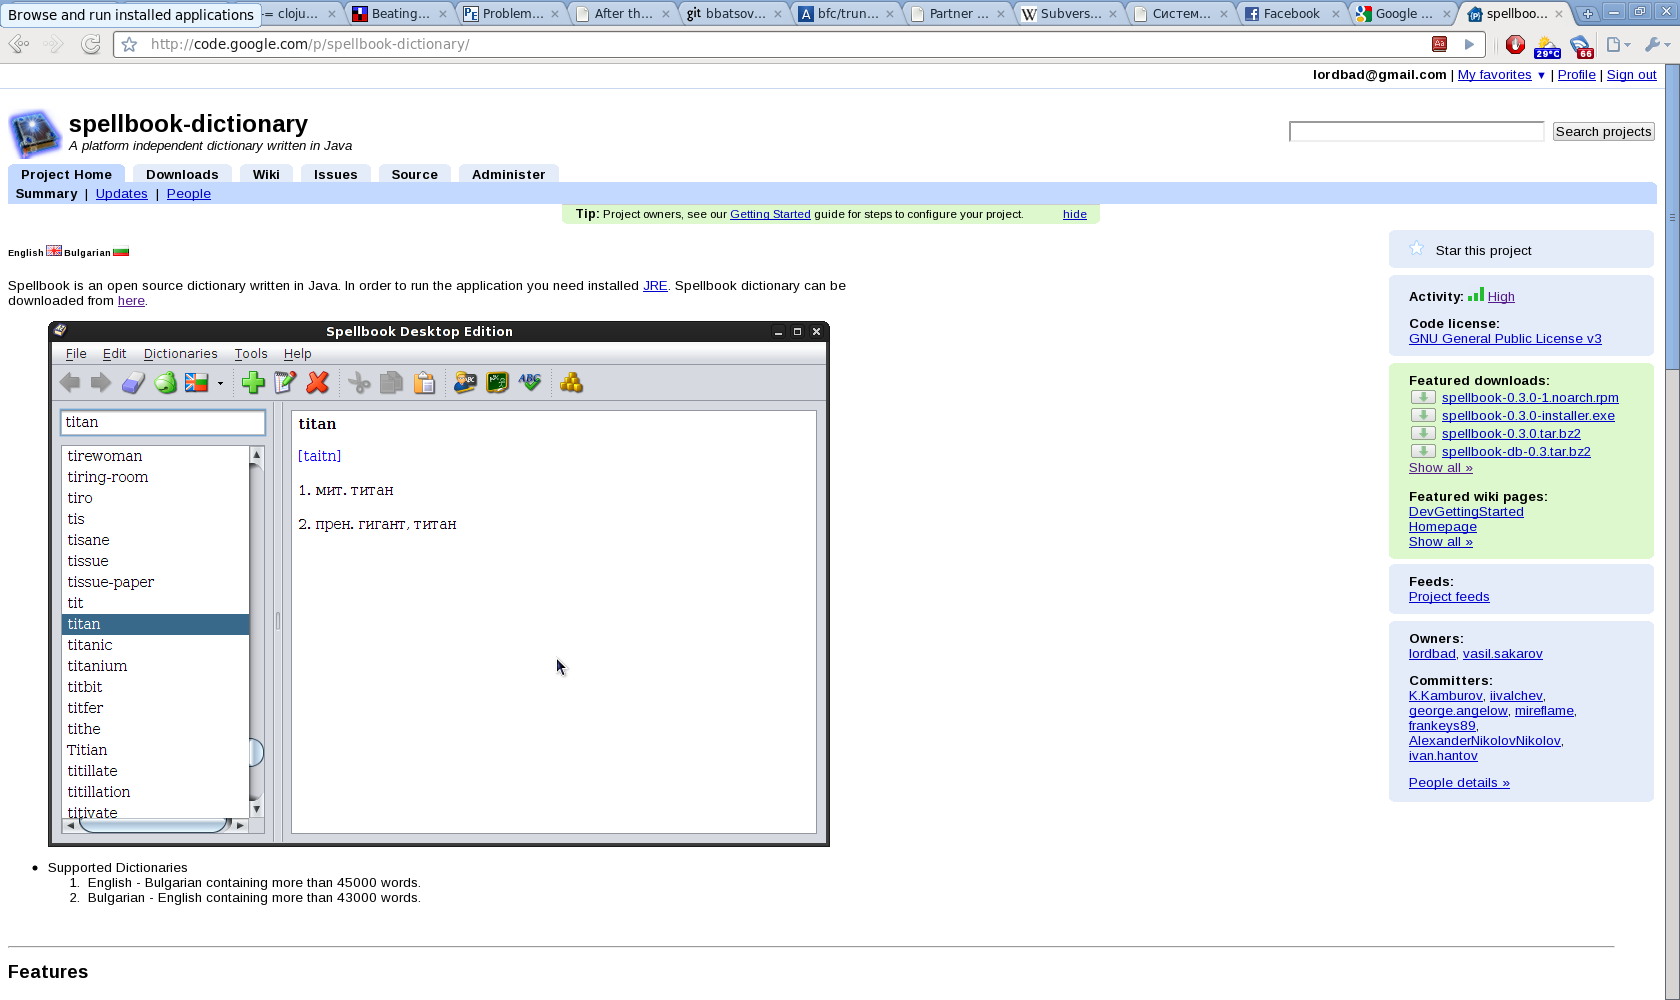
\includegraphics[width=110mm, height=90mm]{images/project-site.png}
\end{figure}

Освен това проекта притежава и дискусионна група в Google Groups -
spellbook-dictionary@googlegroups.com. Това е мястото, където се
обсъждат новите възможности на приложението, както и където формално
се обявява излизането на новите версии.

%%% Local Variables: 
%%% mode: latex
%%% TeX-master: "master"
%%% End: 
